\documentclass[11pt]{report}

% sensible specification of margins, etc.
\usepackage[paperwidth=8.5in,paperheight=11in]{geometry}
\geometry{inner=1.0in, outer=1.5in, top=1.0in, bottom=0.5in,
  includefoot}
\geometry{twoside}

% for displaying graphics
\usepackage[]{graphicx}
% where can I find the graphics that will be imported for this version
\graphicspath{{./figures/}}

% running headers
\usepackage{fancyhdr}
\fancyhead{}
\fancyfoot{}
\fancyhead[CO,CE]{---Draft---}
\fancyhead[LO,RE]{\it Ginga FITS Viewer Manual}
\fancyhead[LE,RO]{\slshape \rightmark}
\fancyfoot[C]{\thepage}
%\fancyfoot[LE,RO] {\slshape \rightmark}
%\fancyfoot[LO,RE] {\slshape \leftmark}

% for Japanese language support, comment out if this causes a problem
\usepackage{xeCJK}
\setCJKmainfont{TakaoMincho}

% use modern and attractive fonts
\usepackage{fontspec}
\setmainfont[Mapping=tex-text]{Times New Roman}
\setsansfont[Mapping=tex-text]{Arial}
%\setmonofont[Scale=0.85]{Courier New}
\setmonofont[]{Courier New}
%% \setmainfont[Mapping=tex-text]{Bitstream Vera Serif}
%% \setsansfont[Mapping=tex-text]{Bitstream Vera Sans}
%% \setmonofont[Scale=0.85]{Bitstream Vera Sans Mono}

% Save space in headings
%% \usepackage[small,compact]{titlesec}
%% \titlespacing{\section}{0pt}{*0}{*0}
%% \titlespacing{\subsection}{0pt}{*0}{*0}
%% \titlespacing{\subsubsection}{0pt}{*0}{*0}

% provides itemize* environment
\usepackage{mdwlist}
% for tables with paragraphs
\usepackage{tabularx}

% for code listings
\usepackage{listings}
\usepackage{color}
\usepackage{textcomp}
\lstset{
	%backgroundcolor=\color{lbcolor},
	tabsize=4,
	%rulecolor=,
	language=Python,
        basicstyle=\scriptsize,
        upquote=true,
        aboveskip={1.5\baselineskip},
        columns=fixed,
        extendedchars=true,
        breaklines=true,
        prebreak = \raisebox{0ex}[0ex][0ex]{\ensuremath{\hookleftarrow}},
        %frame=single,
        showtabs=false,
        showspaces=false,
        showstringspaces=false,
        identifierstyle=\ttfamily,
        keywordstyle=\color[rgb]{0,0,1},
        commentstyle=\color[rgb]{0.9,0.0,0.133},
        stringstyle=\color[rgb]{0.127,0.5126,0.941},
}
\usepackage{verbatim}
\newenvironment{myverbatim}
  {\setlength{\parskip}{0pt}\verbatim}
  {\endverbatim}

%\raggedright

\setlength{\parindent}{0cm}
\setlength{\parskip}{1em plus0.5em minus0.5em}

\setlength{\marginparsep}{0.35in}
\setlength{\marginparwidth}{1.5in}

\title{The Ginga FITS Viewer Manual} 
\author{Eric Jeschke\\
{\tt eric@naoj.org},\\
 (alt) {\tt eric@redskiesatnight.com}\\
\\
Observation Control Software Group\\
Subaru Telescope\\
National Astronomical Observatory of Japan}

\pagestyle{fancy}    


\begin{document} 

\maketitle 

\begin{abstract}
Ginga is a viewer for astronomical data FITS (Flexible Image Transport
System) files.
The Ginga viewer is based on a new FITS display widget which supports 
zooming and panning, color and intensity mapping, a choice of several
automatic cut levels algorithms and canvases for plotting scalable
geometric forms.  In addition to this widget, the fits viewer provides a
flexible plugin framework for extending the viewer with many different
features.  A fairly complete set of standard plugins are provided
for features that we expect from a modern viewer: panning and zooming
windows, star catalog access, cuts, star pick/fwhm, thumbnails, etc.
\end{abstract}

\tableofcontents
\setcounter{tocdepth}{3}

\newpage

%%%%%%%%%%%%%%%%%%%%%%%%%%%%%%%%%%%%%%%%%%%%%%%%%%%%%%%%%%%%% 
\chapter{Introduction}
\label{sh:intro}
\begin{center}
\Huge{銀河}
\end{center}

%%%%%%%%%%%%%%%%%%%%%%%%%%%%%%%%%%%%%%%%%%%%%%%%%%%%%%%%%%%%% 

\section{About}
\label{sec:about}
\emph{Ginga} is a general purpose viewer and tool designed to work
with astronomical data files based on the FITS (Flexible Image Transport
System) file format.  It was written and is maintained by software
engineers at the Subaru Telescope, National Astronomical Observatory of
Japan.

\subsection{Features}
The Ginga viewer centers around a new FITS display widget which supports 
zooming and panning, color and intensity mapping, a choice of several
automatic cut levels algorithms and canvases for plotting scalable
geometric forms.  In addition to this widget, the fits viewer provides a
flexible plugin framework for extending the viewer with many different
features.  A fairly complete set of "standard" plugins are provided
for features that we expect from a modern viewer: panning and zooming
windows, star catalog access, cuts, star pick/fwhm, thumbnails, etc.

\section{Core Concepts}
Ginga operation and documentation is organized around a few core
concepts and associated terminology.  Knowing these may aid in
comprehending the rest of the documentation. 

\subsection{Workspaces}
Ginga has a flexible panel/workspace layout algorithm that allows a
lot of customization into the appearance of the program.  The majority
of the interface is constructed as hierchical series of horizontally or
vertically-adjustable panels.  At the terminus of each panel is a
\emph{workspace}.
Each workspace is typically
implemented by a GUI toolkit container widget such as a notebook widget,
where each item in the workspace is identified by a tab.  Workspaces can
be nested, so a tab might contain yet another nested set of tabs, and so
on\footnote{Note that workspaces may be implemented by several types of 
  container widgets such as fixed position subwindows, sliding panes,
  MDI-style subwindows, etc.  A notebook widget is simply the most
  common (default) case.}. 
Tabs can be freely dragged between workspaces, or out onto the desktop,
forming a new, detached workspace.

In its default configuration, Ginga starts up with a
single row (horizontal) panel of three workspaces, as shown in
Figure \ref{fig:gingadefault}.
This panel is sandwiched vertically between a menu bar and a status bar.

% fig: showing the default configuration
\begin{figure}
  \begin{center}
    \begin{tabular}{c}
      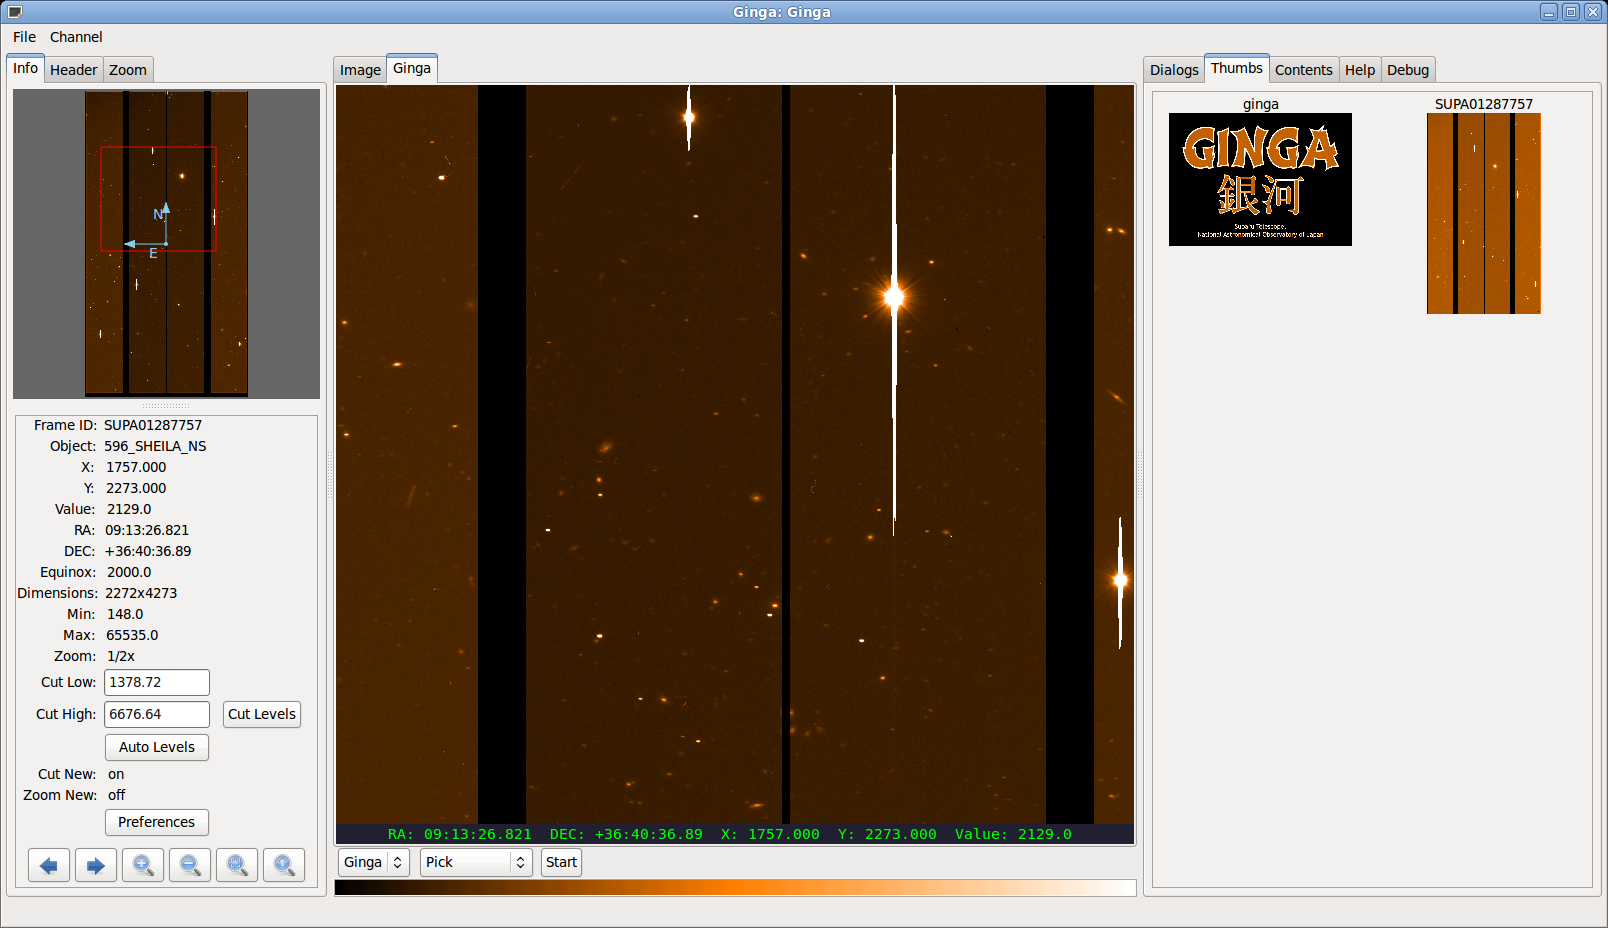
\includegraphics[width=6in]{gingadefault.png}
    \end{tabular}
  \end{center}
  \caption[example] 
%% %>>>> use \label inside caption to get Fig. number with \ref{}
          { \label{fig:gingadefault} 
            A typical Ginga layout.} 
\end{figure} 

The layout of the workspaces is controlled by a table in the Ginga
startup script.  By changing this table the layout can be radically altered.

\subsection{Channels}
Another core tenet of Ginga is that FITS image content is organized
into {\em channels}.  A channel can be thought of as simply a named
category under which similar types of images might be organized.
Examples: 
\begin{itemize*}
\item a channel for each type of instrument at a telescope;
\item a channel for each observation or calibration target;
\item channels based on time or program or proposal identifier;
\item etc.
\end{itemize*}
If no channels are specified when Ginga starts up it simply creates a
default channel named ``Image''.  New channels can be created using the
{\tt Channel/Add channel} menu item.

In the case where multiple channels are present, they are usually visually
organized as tabs within the central workspace of the interface.  To
change channels you simply click on the tab of the channel you want to
view.  There is also a channel selector in the plugin manager toolbar at
the bottom of the center pane.  Using the drop-down menu or by simply
scrolling the mouse wheel on the control you can change the channel.

Channels occupy a flat namespace; i.e. there is no sense of a hierarchy
of channels.
By default, images are loaded into the same channel you are currently
viewing (unless your viewer has been customized to load images according
to special rules).
To keep images organized, simply change to the desired channel before
opening a new image. 

\subsection{Plugins}
Most functionality in Ginga is achieved through the use of a plugin
architecture.
In this manual we will also use the word {\em operation} to describe activating
a plugin.  For example, a pick operation would invoke and use the Pick
plugin.  The plugins are each described in more detail in Chapter 
\ref{ch:plugins}.  Plugins are written as encapsulated Python modules
that are loaded dynamically when Ginga starts.  There is an API for
programming plugins (see Chapter \ref{ch:plugins}).  

A plugins may or may not have an associated Graphical User Interface (GUI).
For those that do have a visible interface, the Ginga startup script
can map them to certain workspaces.  By manipulating this mapping (along
with the workspace layout) extremely customized and flexible layouts can
be achieved.  
In Figure \ref{fig:gingadefault} the left workspace contains three
global plugin UIs: the Info, Header and Zoom panes.  The middle workspace
holds all the viewing panes for each channel.  The right workspace has
the Dialogs, Thumbs, Contents and Help panes.  The operation of these
plugins is described in Chapter \ref{ch:plugins}. 

\section{General operation}
\label{sec:generalop}

\subsection{Terminology}
In this manual we will use the following terms to describe operations
with the mouse:
\begin{itemize*}
\item \emph{Click} or \emph{Left-click} means to click on an item with
  the left mouse button;
\item \emph{Drag} or \emph{Left-drag} means to click, hold and drag with
  the left mouse button;
\item \emph{Scroll} means to scroll with the middle mouse wheel;
\item \emph{Scroll-click} means to click with the middle mouse wheel/button;
\item \emph{Scroll-drag} means to click, hold and drag with the middle
  mouse wheel/button; 
\item \emph{Right-click} means to click on an item with the right mouse
  button; 
\item \emph{Right-drag} means to click, hold and drag with the right
  mouse button.
\end{itemize*}

Mouse operations are also modified by the keyboard buttons {\tt Shift}
and {\tt Ctrl}.  \emph{Shift-click} means to press \emph{and hold} the
{\tt Shift} key while clicking with left mouse button,
\emph{Shift-right-click} is the same using the right mouse button,
etc.
Some mouse-controlled operations in Ginga are initiated by a key stroke.
In these cases the key is pressed and released (not held), and then the
mouse is used to control the operation.  Such operations are either
terminated by releasing the mouse button (if the operation employs a
drag), clicking on the image or pressing the {\tt Esc} key (if not a
drag operation).

\subsection{Loading a FITS image file}
There are several ways to load a file into Ginga.  Perhaps the canonical
way is to use the {\tt Load Image} entry from the {\tt File} menu on the
main menu bar at the top of the window.  This opens a standard file
dialog popup window where you can navigate to the file you wish to load.

Another way is to invoke the FBrowser plugin, which opens in the Dialogs
tab.  The plugin pane shows file and folder contents and allows
navigation up and down the filesystem hierarchy by double-clicking on
folder names.   Simply navigate to the location of the FITS file and
double-click on the file name to load it.

Ginga also supports drag-and-drop in a typical desktop Linux
environment, so you can simply drag and drop files from a graphical file
manager such as nautilus onto the main FITS viewing pane to load the image.

\subsection{Zooming and panning}
The FITS widget used throughout most of the Ginga panels has built-in
support for zooming and panning.  Appendix \ref{app:mousekbdref} has the
complete listing of default keyboard and mouse bindings.  
Briefly, the scroll wheel of the mouse can be used to zoom in and out,
along with the {\tt +} and {\tt -} keys.  The backquote key will fit the
image to the window.

When zoomed in, panning is enabled.  Panning takes two forms.
\emph{Free panning} allows scrolling around the entire image by mapping
the entire image boundaries to the window boundaries.  For example,
moving the mouse to the upper right-hand corner of the window will pan to
the upper right hand corner of the image, etc.  Scroll-drag to free pan,
or press and release {\tt q} and then move the mouse around the window
(left-click to stop a {\tt q}-initiated free pan).
\emph{Proportional panning} pans the image in direct proportion to the
distance the mouse is moved; a common idiom is dragging the image canvas in
the direction you want to move it under the window.  To utilize a
proportional pan, Ctrl-drag the canvas.  The Pan plugin (usually
embedded under the {\tt Info} tab) shows the outline of the current pan
position as a rectangle on a small version of the whole image. 
Dragging this outline will also pan the image in the main window.

Panning in Ginga is based on dimensional pan factors, collectively known
as the \emph{pan position}.  The pan position determines what Ginga will
try to keep in the middle of the window as the image is zoomed.  
When zoomed out, one can Shift-click on a particular point in the image
(or press the {\tt p} key while hovering over a spot),
setting the pan position.  Zooming in afterward will keep the pan
position as much as possible in the center of the window.  The pan
position may also be set by certain plugins, such as Pick.

Ginga has an auto zoom feature to automatically fit newly loaded images
to the window.  See section \ref{pref:autozoom} for details.

\subsection{Setting cut levels}

Ginga has an auto cuts feature to automatically set cut levels on newly
loaded images.  See section \ref{pref:autocuts} for details.

\subsection{Manipulating the color map}


%%%%%%%%%%%%%%%%%%%%%%%%%%%%%%%%%%%%%%%%%%%%%%%%%%%%%%%%%%%%% 
\chapter{Plugins}
\label{ch:plugins}
%%%%%%%%%%%%%%%%%%%%%%%%%%%%%%%%%%%%%%%%%%%%%%%%%%%%%%%%%%%%% 
Ginga is written so that most of the functionality of the program is
achieved through the use of plugins.  This modular approach allows a
large degree of flexiblity and customization, as well as making overall
design and maintenance of the program simpler.

Plugins are divided into two types: global and local.  A global plugin
has a single instance shared by all channels, while a local plugin
creates a unique instance for each channel.  If you switch channels, a
global plugin will respond to the change by updating itself,
while a local plugin will remain unchanged if the channel is switched,
because its operation is specific to a given channel.

This chapter describes the set of plugins that come with Ginga.  Those
interested in writing their own custom plugins should refer to chapter
\ref{ch:writingplugins}. 

\section{Global plugins}

\subsection{Pan}
The Pan plugin provides a small panning image that gives an overall
``birds-eye'' view of the channel image that last had the focus.  If the
channel image is zoomed in 2X or greater then the pan region is shown
graphically in the Pan image by a rectangle.  The channel image can be
panned by clicking and/or dragging to place the rectangle.  You can also
use the scroll wheel in the Pan image to zoom the channel image.

The color/intensity map and cut levels of the Pan image are updated
when they are changed in the corresponding channel image.
The Pan image also displays the World Coordinate System compass, if
valid WCS metadata is present in the FITS HDU being viewed in the
channel.

\subsection{Info}
The Info plugin provides a pane of commonly useful metadata about the
associated channel image.  Common information includes some
FITS header values, the equinox, dimensions of the image, minimum and
maximum values and the zoom level.  As the cursor is moved around the
image, the X, Y, Value, RA and DEC values are updated to reflect the
value under the cursor.

At the bottom of the Info interface are the cut levels controls. Here
the low and high cut levels are shown and can be adjusted.  Finally,
there is a Preferences button that will take the user quickly to the
Preferences plugin for the channel.

The Pan and Info plugins are typically combined under the Info tab in
the user interface.  Below the Info plugin appear several buttons that
can be used to zoom the image or to navigate between images in the
history of the current channel.

\subsection{Header}
The Header plugin shows the FITS keyword metadata from the image.
Initially only the primary HDU metadata is shown.  However, in
conjunction with the MultiDim plugin the metadata for other HDUs will be
shown.  See the MultiDim plugin description for details.

Clicking on a column header will sort the table by values in that
column, which may be useful for quickly locating a particular keyword.

\subsection{Zoom}
The Zoom plugin shows an enlarged image of a cutout region centered
under the cursor position in the associated channel image.  As the
cursor is moved around the image the zoom image updates to allow close
inspection of the pixels or precise control in conjunction with other
plugin operations.

The size of the cutout radius can be adjusted by the slider below the
zoom image labeled ``Zoom Radius''. The default radius is 30 pixels,
making a 61x61 zoom image.  The magnification can be changed by
adjusting the ``Zoom Amount'' slider.
Above zero, the zoom range corresponds to logical increments: 1=1X,
2=2X, etc.  The zoom scale is discontinuous at the 0 and -1 settings,
which are equivalent to 1X.  Settings below -1 correspond to zooming out,
e.g. -2=1/2, -3=1/3, etc. 

Two modes of operation are possible: absolute and relative zoom.  In
absolute mode, the zoom amount controls exactly the zoom level shown in
the cutout: for example, the channel image may be zoomed into 10X, but
the zoom image will only show a 3X image if the zoom amount is set to
3X.
In relative mode, the zoom amount setting is interpreted as relative to
the zoom setting of the channel image.  If the zoom amount is set to 3X
and the channel image is zoomed to 10X then the zoom image shown will be
10+3=13X.  Note that the zoom amount setting can be negative, so a
setting of -3X with a 10X zoom in the channel image will produce a
10-3=7X zoom image.
In both modes the minimum and maximum zoom level of the zoom image is
limited by the Min Zoom and Max Zoom settings, which are
user-adjustable.  

\subsection{Thumbs}
The Thumbs plugin provides an index of all images viewed since the
program was started.  Clicking on a thumbnail navigates you directly to
that image.  Thumbs appear in cronological viewing history, with the
newest images at the bottom and the oldest at the top.  Hovering the
cursor over a thumbnail will show a tooltip that contains a couple of
useful pieces of metadata from the image.

\subsection{Contents}
The Contents plugin provides a table of contents like interface for all
the images viewed since the program was started.  Unlike Thumbs,
Contents is sorted by channel, and then by image name.  The contents
also shows some common metadata from the image.

\section{Local plugins}

An {\em operation} is the activation of a local plugin to perform some
function.  Operations can the started and controlled in two ways:
graphically, or using the keyboard shortcuts.  The plugin manager
toolbar at the bottom of the center pane is the graphical way to start
an operation.  


\subsection{Pick}
\subsection{Ruler}
\subsection{MultiDim}
\subsection{Cuts}
\subsection{Histogram}
\subsection{PixTable}
\subsection{Preferences}

\label{pref:autozoom}
Ginga can automatically set the zoom level to fit the window when you
switch images; 
for example, when a new image is loaded into a channel or you click the
thumbnail of an old image.
This setting is on a per-channel basis and is governed by the ``Zoom
New'' setting with three possible values: on, override, and off.  
In the \emph{on} mode, the switched image is always zoomed to fit.  In the 
\emph{off} mode, the current zoom settings are applied to the new image.
In \emph{override} mode, images are automatically fitted until the zoom is
changed manually--then the mode automatically changes to \emph{off}.
Override mode can be re-enabled from off mode by a keypress--see
Appendix \ref{app:mousekbdref} for the default key binding.

\label{pref:autocuts}
Ginga can automatically set cut levels when you switch images;
for example, when a new image is loaded into a channel or you click the
thumbnail of an old image.
This setting is on a per-channel basis, and is governed by three
possible values for the ``Cut New'' setting (on, override, and off).
%% The idea of the ``Use saved cuts'' preference comes from the notion that
%% if you previously manually set the cut levels on an image then you
%% probably want to use the same cut levels if you visit that same image again.  
%% So if the switched image is already loaded (e.g. you clicked a thumbnail of
%% an older image) \emph{and} a \emph{manual} cut levels operation was
%% previously applied to that image \emph{and} the use saved cuts checkbox
%% is checked, then the previously saved cut levels for that image will be
%% used.
In the \emph{on} mode, an auto cut levels is always applied to the
new image.  
In the \emph{off} mode, the current cut levels are applied to the new image.
In \emph{override} mode, images are automatically cut until the cut levels are
changed manually--then the mode automatically changes to \emph{off}.

\subsection{Catalog}
\subsection{Drawing}
\subsection{FBrowser}
\subsection{WBrowser}

\chapter{Customizing Ginga}
\label{ch:customizing}
This chapter explains how you can customize Ginga in various ways.

\section{Workspace configuration}
\label{sec:workspaceconfig}
Ginga has a flexible table-driven layout scheme for dynamically creating
workspaces and mapping the plugins to workspaces.  By changing a couple
of tables you can change the way Ginga looks and presents its content. 
If you examine the top-level startup script {\tt ginga.py} you will find
the tables: {\tt default\_layout}, {\tt global\_plugins} and
{\tt local\_plugins}.
global\_plugins and local_\plugins define the mapping of plugins to
workspaces and the titles on the tabs in the workspaces (if the
workspace has tabs--some don't).  
Here is an example of these two tables:
\begin{lstlisting}
global_plugins = [
    Bunch(module='Pan', tab='Pan', ws='uleft', raisekey='i'),
    Bunch(module='Info', tab='Info', ws='lleft', raisekey='i'),
    Bunch(module='Header', tab='Header', ws='left', raisekey='h'),
    Bunch(module='Zoom', tab='Zoom', ws='left', raisekey='z'),
    Bunch(module='Thumbs', tab='Thumbs', ws='right', raisekey='t'),
    Bunch(module='Contents', tab='Contents', ws='right', raisekey='c'),
    Bunch(module='WBrowser', tab='Help', ws='right', raisekey='?'),
    Bunch(module='Errors', tab='Errors', ws='right'),
    Bunch(module='Log', tab='Log', ws='right'),
    Bunch(module='Debug', tab='Debug', ws='right'),
    ]

local_plugins = [
    Bunch(module='Pick', ws='dialogs', shortkey='f1'),
    Bunch(module='Ruler', ws='dialogs', shortkey='f2'),
    Bunch(module='MultiDim', ws='dialogs', shortkey='f4'), 
    Bunch(module='Cuts', ws='dialogs', shortkey='f5'),
    Bunch(module='Histogram', ws='dialogs', shortkey='f6'),
    Bunch(module='PixTable', ws='dialogs', shortkey='f7'),
    Bunch(module='Preferences', ws='dialogs', shortkey='f9'),
    Bunch(module='Catalogs', ws='dialogs', shortkey='f10'),
    Bunch(module='Drawing', ws='dialogs', shortkey='f11'),
    Bunch(module='FBrowser', ws='dialogs', shortkey='f12'), 
    ]
\end{lstlisting}
The format of this table is simply a series of tuples''bunches''.
In the case of global\_plugins, each bunch specifies a module 
a title for the tab, the workspace that it should occupy, and an
optional key to raise that tab when pressed.
We can see that the ``Pan'' plugin will occupy the ``uleft'' workspace
and have a tab name of ``Pan'' (if that workspace has tabs).

Next we look at the default\_layout table:
\begin{lstlisting}
default_layout = ['hpanel', {},
                  ['ws', dict(name='left', width=320),
                   # (tabname, layout), ...
                   [("Info", ['vpanel', {},
                              ['ws', dict(name='uleft', height=300,
                                          show_tabs=False)],
                              ['ws', dict(name='lleft', height=430,
                                          show_tabs=False)],
                              ]
                     )]
                     ],
                  ['vbox', dict(name='main', width=700)],
                  ['ws', dict(name='right', width=400),
                   # (tabname, layout), ...
                   [("Dialogs", ['ws', dict(name='dialogs')
                                 ]
                     )]
                    ],
                  ]
\end{lstlisting}
This table defines how many workspaces we will have, their
characteristics, how they are organized, and their names.
The table consists again of a series of sublists or tuples, but in this
case they can be nested.
The first item in a sublist indicates the type of the container to be
constructed.  The following types are available:
\begin{itemize}
\item hpanel -- a horizontal panel of containers, with handles to size them
\item vpanel -- a vertical panel of containers, with handles to size
  them
\item hbox -- a horizontal panel of containers of fixed size
\item vbox -- a vertical panel of containers of fixed size
\item ws -- a workspace that allows a plugin gui or other items, usually
  implemented by a notebook-type widget
\item widget -- a preconstructed widget passed in
\end{itemize}
In every case the second item in the sublist is a dictionary that
provides some optional parameters that modify the characteristics of the
container.
If there is no need to override the default parameters the dictionary
can simply be empty.
The optional third and following items are specifications for nested
content.

All types of containers honor the following parameters:
\begin{itemize}
\item width -- can specify a desired width in pixels for the container.
\item height -- can specify a desired height in pixels for the container.
\item name -- specifies a mapping of a name to the created container
  widget.  The name is important especially for workspaces, as they may
  be referred to in the default\_tabs table.
\end{itemize}

In the above example, we define a top-level horizontal panel of three
containers: a workspace named ``left'' with a width of 320 pixels, a
vertical fixed container named ``main'' with a width of 700 pixels and a
workspace called ``right'' with a width of 400 pixels.  The ``left''
workspace is pre-populated with an ``Info'' tab containing a vertical
panel of two workspaces: ``uleft'' and ``lleft'' with heights of 300 and
430 pixels, respectively, and neither one should show tabs.  The ``right''
workspace is pre-populated with a ``Dialogs'' tab containing an empty
workspace.  Looking back at the  default\_tabs table you can now more 
clearly see how the mapping of plugins to workspaces is handled through
the names.

Ginga uses some container names in special ways.
For example, the ``main'' container is populated by Ginga with the tabs
for each channel, and the ``dialogs'' workspace is where all of the
local plugins are instantiated (when activated).
These two names should at least be defined somewhere in default\_layout.

\section{Writing a global plugin}
\label{sec:globalplugins}
Global plugins are basically treated like mini programs that get loaded
into Ginga and are started when the program starts\footnote{If the
  plugin is not listed in the default\_tabs table described in section
  \ref{sec:workspaceconfig} it won't be started at program startup.}.
A global plugin does not need to have a user interface associated with
it.  

Global plugins are best suited for adding features to Ginga that
should operate ``across channels''; i.e. some visible interface that
continuously updates itself in response to events happening in the
viewer.

The API for a global plugin is pretty simple.  This template shows the
relevant class definition:
\begin{lstlisting}
class Foo(GingaPlugin.GlobalPlugin):
    """
    NOTE: *** All these methods are running in the GUI thread, unless
    otherwise noted. Do not block!! ***  
    """

    def __init__(self, fv):
        super(Foo, self).__init__(fv)

        # Hereafter, in this object we can refer to:
        # self.fv -- the main Ginga control object
        # self.logger -- a logger

    def initialize(self, container):
        """This method will be called with a container widget if the global
        plugin was requested to be loaded into a workspace.  The plugin should
        construct its GUI and pack it into the container.
        """
        pass

   def start(self):
        """This method is reserved for future use.
        """
        pass

   def stop(self):
        """This method is reserved for future use.
        """
        pass
\end{lstlisting}
There is the object constructor, an {\tt initialize} method and 
{\tt start} and {\tt stop} methods.  
Global plugins register with the main ginga object for events they
are interested in, like when a channel is added, or a new image arrives
in a channel, and define their own callbacks to deal with them.  This is
typically done in the constructor, although it can also be done in the
{\tt initialize} method.  The start and stop methods are currently 
reserved for future use and can be omitted. 

The best way to learn how a global plugin interacts with the main Ginga
control object (represented by the {\tt fv} parameter in the
constructor) is to examine some of the global plugins that ship with
Ginga.  Start with a simple one, like Header, and work up to more
complicated examples like Info.

\section{Writing a local plugin}
\label{sec:localplugins}
Local plugins are also more or less independent modules that are loaded
into Ginga at program startup, but there is a unique instance of a local
plugin for each channel.  Local plugins are also more tightly controlled
by Ginga: they create their user interface (if any) when the plugin
is activated, and it disappears when the plugin is deactivated.
Furthermore, while the plugin is activated it may lose or regain the
focus, which generally serves to multiplex the keyboard and mouse
operations amongst the different active local plugins.  
Local plugins are activated, deactivated and focus-controlled via the 
plugin manager bar that appears at the bottom of the main FITS window.

Here is a template for a local plugin.  As you can see, the API is a
little more complicated than for a global plugin, but not by much.
\begin{lstlisting}
class Goo(GingaPlugin.LocalPlugin):
    """
    NOTE: *** All these methods are running in the GUI thread, unless
    otherwise noted. Do not block!! ***  
    """

    def __init__(self, fv, fitsimage):
        super(Goo, self).__init__(fv, fitsimage)

        # Hereafter, in this object we can refer to:
        # self.fv -- the main Ginga control object
        # self.fitsimage -- the channel viewer object we are associated with
        # self.logger -- a logger

    # def build_gui(self, container):
    #     """If a plugin defines this method, it will be called with a
    #     container object in which to build its GUI. It should finish
    #     by packing into this container.  This will be called every
    #     time the local plugin is activated.
    #     """
    #     pass

    def start(self):
        """This method is called just after build_gui() when the plugin is
        activated.
        """
        pass
        
    def stop(self):
        """This method is called when the plugin is deactivated.
        """
        pass

    def pause(self):
        """This method is called when the plugin is defocused.  The plugin
        should disable any user input that it responds to.
        """
        pass

    def resume(self):
        """This method is called when the plugin is focused.  The plugin
        should enable any user input that it responds to.
        """
        pass

    def redo(self):
        """This method is called when a new image arrives in the channel
        associated with the plugin.  It can optionally redo whatever operation
        it is doing.
        """
        pass
\end{lstlisting}

The best way to learn how a local plugin interacts with the main Ginga
control object (the {\tt fv} parameter in the constructor) and the local
channel image ({\tt fitsimage}) is to examine some of the local plugins
that ship with Ginga.  Start with a simple one, like Ruler or Drawing,
and work up to more complicated examples like Pick or Catalogs.

\section{Remote Control}
\label{sec:remotecontrol}
You may find that you have a need to control Ginga remotely.  For
example, you want to invoke the loading of images, or performing
operations on images, etc.  Like many other aspects, Ginga delegates this
task to a plugin: RC.  
Because remote control of Ginga is handled by a plugin, you can easily
change the types of operations that can be done, or completely change
the protocol used.

The remote control module is not loaded by default.  To load it, specify
the command line option:
\begin{verbatim}
--modules=RC
\end{verbatim}

You can then control Ginga from the {\tt grc\.py} program located in the 
{\tt util} directory.  Some examples:
\begin{verbatim}
 Create a new channel:
 $ ./grc.py add_channel FOO
 
 Load a file:
 $ ./grc.py display_fitsfile FOO /home/eric/testdata/SPCAM/SUPA01118797.fits False

 Load a file, controlled from a different host:
 $ ./grc.py --host=bar --port=9000 display_fitsfile FOO /home/eric/testdata/SPCAM/SUPA01118797.fits False

 Cut levels:
 $ ./grc.py cut_levels FOO 163 1300

 Auto cut levels:
 $ ./grc.py autocuts FOO

 Zoom to a specific level:
 ./grc.py -- zoom FOO -7
 
 Zoom to fit:
 ./grc.py zoom_fit FOO
 
 Transform:
 ./grc.py transform FOO 1 0 1
\end{verbatim}

\chapter{Ginga Programming Internals}
\label{ch:internals}
This chapter explains the secret inner workings of Ginga and its widgets
so that you can subclass them and use them in your own applications.

\bf{TBD}

\section{Architecture}

\bf{TBD}

%%%%%%%%%%%%%%%%%%%%%%%%%%%%%%%%%%%%%%%%%%%%%%%%%%%%
\appendix    %>>>> this command starts appendixes
%%%%%%%%%%%%%%%%%%%%%%%%%%%%%%%%%%%%%%%%%%%%%%%%%%%%

\chapter{Keyboard and Mouse Quick Reference}
\label{app:mousekbdref}

\section{Main image window}
These keyboard and mouse operations are available when the main image
window has the focus.

\subsection{Panning and Zooming commands}
\begin{tabularx}{\textwidth}{lX}
Scroll wheel turned & Zoom in or out \\
Digit ({\tt 1234567890}) & Zoom image to 1X, 2X, ..., 9X, 10X \\
Shift + Digit & Zoom image to 1/2X, 1/3X, ..., 1/9X, 1/10X \\
Backquote (\`{}) & Zoom image to fit window \\
Minus, Underscore ({\tt -\textunderscore{}}) & Zoom out \\
Equals, Plus ({\tt =+}) & Zoom in \\
Middle (scroll) button drag & Pan image freely (when zoomed in) \\
{\tt p} & Set pan position for zooming \\
Shift + Left click & Set pan position for zooming \\
{\tt q} & Pan image freely (when zoomed in); move mouse (no button press); left click to terminate) \\
Ctrl + Left drag & Proportional pan (press and drag left mouse button) \\
apostrophe ({\tt '}) & Set autozoom for new images to {\em override} \\
doublequote ({\tt ''}) & Set autozoom for new images to {\em on} \\
\end{tabularx}

\subsection{Cut levels and colormap commands}
\begin{tabularx}{\textwidth}{lX}
{\tt a} & Auto cut levels \\
comma, left angle ({\tt ,\textgreater{}}) & Interactive cut low (with left mouse button) \\ 
period, right angle ({\tt .\textless{}}) & Interactive cut high (with left mouse
button) \\ 
slash ({\tt /}) & Interactive shift colormap (with left mouse button) \\
semicolon ({\tt ;}) & Set autocuts for new images to {\em override} \\
colon ({\tt :}) & Set autocuts for new images to {\em on} \\
Ctrl + Scroll wheel turned & Adjust \emph{both} high and low cut levels
(coarse adjustment) \\
Shift + Scroll wheel turned & Adjust \emph{both} high and low cut levels
(fine adjustment) \\
\end{tabularx}

\subsection{Transform commands}
\begin{tabularx}{\textwidth}{lX}
Left bracket ({\tt [}) & Flip image in X \\
Left brace ({\tt \textbraceleft{}}) & Restore image in X \\
Right bracket ({\tt ]}) & Flip image in Y \\
Right brace ({\tt \textbraceright{}}) & Restore image in Y \\
Backslash ({\tt \textbackslash{}}) & Swap X and Y axes \\
Vertical bar ({\tt \textbar{}}) & Restore X and Y axes \\
\end{tabularx}

\subsection{Tab Navigation}
\begin{tabularx}{\textwidth}{lX}
{\tt i} & Raise Info tab \\
{\tt h} & Raise Header tab \\
{\tt z} & Raise Zoom tab \\
{\tt d} & Raise Dialogs tab \\
{\tt t} & Raise Thumbs tab \\
{\tt c} & Raise Contents tab \\
{\tt ?} & Raise Help tab \\
\end{tabularx}

\subsection{Plugins}
\begin{tabularx}{\textwidth}{llX}
Escape & Stop current plugin operation & \\
{\tt F1} & Start Pick & Stellar evaluation \\
{\tt F2} & Start Ruler & Measure distances \\
{\tt F3} & (Reserved for future use) & \\
{\tt F4} & Start MultiDim & Browse HDUs and image slices \\
{\tt F5} & Start Cuts & Graph pixel values along a line \\
{\tt F6} & Start Histogram & Graph pixel values in a region \\
{\tt F7} & Start PixTable & Show maxtrix of pixel values around cursor \\
{\tt F8} & (Reserved for future use) & \\
{\tt F9} & Start Preferences & Set preferences for a channel \\
{\tt F10} & Start Catalog & Access image and star catalogs \\
{\tt F11} & Start Drawing & Draw graphics on an image \\
{\tt F12} & Start FBrowser & Browse and load files \\
\end{tabularx}

If there are one or more plugins active, additional mouse or keyboard
bindings may be present.  In general, the left mouse button is used to
select, pick or move, and the right mouse button is used to draw a
shape for the operation.  
On the Mac, control + mouse button can also be used to draw or right click.

\chapter{Miscellanea}
\section{Etymology}
``Ginga'' is the romanized spelling of the Japanese word ``銀河''
(hiragana: ぎんが), meaning ``galaxy'' (in general) and, more familiarly,
the Milky Way.  This viewer was written by software engineers at Subaru
Telescope, National Astronomical Observatory of Japan--thus the
connection. 

\section{Pronunciation}
Ginga the viewer may be pronounced ``ging-ga'' (proper japanese) or
``jing-ga'' (perhaps easier for western tongues).  The latter
pronunciation has meaning in the Brazilian dance/martial art
\emph{capoeira}: a fundamental rocking or back and forth swinging
motion.
Note: pronunciation as ``gin-ja'' is particularly bad form!

\end{document} 
